\documentclass[paper=a4, fontsize=11pt]{scrartcl} % A4 paper and 11pt font size
\usepackage{./../usfassignment}
\settitle{Assignment 11}
\setauthor{Wanzhang Sheng}
\setcourse{CS673: Graduate Algorithms}

\begin{document}

\maketitle % Print the title

% -----------------------------------------------------------------------------
% PROBLEM 1
% -----------------------------------------------------------------------------
\section{}

\begin{fancyquotes}
  Professor Adam has two children who unfortunately, dislike each
  other. The problem is so severe that not only do they refuse to walk
  to school together, but in fact each one refuses to walk on any
  block that the other child has stepped on that day. The children
  have no problem with their paths crossing at a corner. Fortunately
  both the professor's house and the school are on corners, but beyond
  that he is not sure if it is going to be possible to send both of
  his children to the same school. The professor has a map of his
  town. Show how to formulate the problem of determining if both his
  children can go the same school as a maximum flow problem.
\end{fancyquotes}

Change the map into a directed graph, the capacity of each edge is 1.
Make the source vertex be the home, and the sink vertex be the school.
Find the maximum flow of the graph.
If the maximum flow is at least 2, then it's possible. Otherwise it's
impossible.

\pagebreak

% -----------------------------------------------------------------------------
% PROBLEM 2
% -----------------------------------------------------------------------------
\section{}

\begin{fancyquotes}
   (8 points) Exercise 26.2--9 Edge connectivity

   The edge connectivity of an undirected graph is the minimum number
   $k$ of edges that must be removed to disconnect the graph. Show how
   the edge connectivity of an undirected graph $G = (V, E)$ can be
   determined by running a maximum-flow algorithm on at most $|V|$
   flow networks, each having $O(|V|)$ vertices and $O(|E|)$ edges.
\end{fancyquotes}

Change the undirected graph into a directed graph which each edge has
capacity 1.
Specify a vertex as the source vertex.
Run $|V|$ times maximum flow with each other vertices as the sink
vertex.
Return the minimal one in the $|V|$ maximum flows.
This is the connectivity of the graph.

For the flow network with the minimal flow, there exists a cut which
the edges on the cut are all full. Otherwise you can still increase
the flow cross the cut.

Since all the edges have capacity 1, the amount of the maximum flow is
the number of the edges to remove.

\pagebreak

% -----------------------------------------------------------------------------
% PROBLEM 3
% -----------------------------------------------------------------------------
\section{}

\begin{fancyquotes}
  Problem 33--3 Ghostbusters \& Ghosts

  A group of $n$ ghostbusters is battling $n$ ghosts. Each Ghostbuster
  is armed with a proton pack, which shoots a stream at a ghost,
  eradicating it. A stream goes in a straight line and terminates when
  it hits a ghost. The Ghostbusters decide upon the following
  strategy. They will pair off with the ghosts, forming $n$
  Ghostbuster-ghost pairs, and then simultaneously each Ghostbuster
  will shoot a stream at his chosen ghost. As we all know, it is very
  dangerous to let the streams cross, and so the Ghostbusters must
  choose parings for which no streams will cross. Assume that the
  position of each ghost and Ghostbuster is a fixed point in the
  plane, and that no three positions are collinear.
\end{fancyquotes}

\subsection{}
\label{sub:GGsame}

\begin{fancyquotes}
  (8 points) Argue that there exists a line passing through one
  Ghostbuster and one ghost such that the number of Ghostbusters on
  one side of the line equals the number of ghosts on the same side
  of the line. Describe how to find a line in $O(n\lg{n})$ time.
\end{fancyquotes}

Color all the Ghostbuster point as black, and all the Ghost as
white.

Sort all the points in the $x$ coordinate in $O(n\lg{n})$, pick the
point $S$ with the minimal $x$.
Draw lines between $S$ and other points, sort them as a array $T$ by
the angle with the $x$ coordinate in $O(n\lg{n})$.

Scan the points in $T$, count the difference between the black and
white in $O(n)$. Output it when it's $0$.

To prove we can always get the answer,
pick the points with max and min angles as $T_1, T_2$.

If $T_1$ or $T_2$ has different color with $S$, pick the line with
it and $S$ as the result, since there are $n-1$ Ghosts and
Ghostbusters on one side.

If $T_1, T_2$ have the same color with $S$, assume they're black.
The difference between black and white at the beginning of the scan is
$1-0=1$.
But at the end of the scan, the last one is also black. The
difference between black and white is $(n-1)-(n)=-1$.
Since no three positions are collinear, everytime you can only meet
one point and change the difference by $1$.
So there has to be some point whose color is white in the middle
changes the difference between black and white from positive to
$0$. Which is the answer and the color of the point is white.

The total time cost is $O(n\lg{n}+n\lg{n}+n)=O(n\lg{n})$

\subsection{}

\begin{fancyquotes}
  (4 points) Give an $O(n^2\lg{n})$ time algorithm to pair
  Ghostbusters and ghosts in such a way that no streams cross.
\end{fancyquotes}

Use the algorithm in~\ref{sub:GGsame} to find the pair who seperate
the points into two parts which inside has the same number of the
Ghostbusters and the Ghosts in $O(n\lg{n})$. Solve the subproblems.
Time cost is $T(n) = n\lg{n}+2\times T(\frac{n-1}{2}) = O(n^2\lg{n})$.
So total time cost is $O(n^2\lg{n})$.

\pagebreak


% -----------------------------------------------------------------------------
% PROBLEM 4
% -----------------------------------------------------------------------------
\section{}

\begin{fancyquotes}
   (8 points) Exercise 32.1--4 Gap Character Suppose

   we allow the patern $P$ to contain occurances of a gap character
   $\diamond$ that can match an arbitrary string of characters (even
   one of zero length). For example, the pattern $ab\diamond
   ba\diamond c$ occurs in the text $cabccbacbacab$ as $abccbacbacab$
   and as $abccbacbac$. Note that the gap character may occur an
   arbitrary number of times in the pattern but is assumed not to
   appear in the text. Give a polynomial-time algorithm to determine
   if such a pattern $P$ occurs in a given text $T$, and analyze the
   running time of your algorithm. Note that you do not need to find
   all occurances, you just need to determine if the pattern occurs a
   all. Give pseudocode.
\end{fancyquotes}

Split the pattern $P$ by $\diamond$ into a array of strings.
Determine the first position match the first string, character by character.
Then detemine the first position match the second string from the
previous position.
Repeat until all the strings are matched then return yes, or reach the
end of the $T$ then return no.

\begin{algorithm}[H]
  \SetKwProg{Fn}{Function}{}{end}
  \Fn{\textsc{match}{(T, P)}}{
    strs = P.splits('$\diamond$') \;
    position = 0 \;
    \For{str in strs}{
      \tcc{From `position' on the first match of `str' in `T'}
      first\_match = first\_match\_with\_offset(T, str, position) \;
      \eIf{first\_match.success?}{
        position = first\_match.position \;
      }{
        return false \;
      }
    }
    return true \;
  }
  \caption{Determine if P matches T.}
\end{algorithm}

Every position in $P$ will only be determin once.
And each time needs $O(|P|)$ at most.
So, the time cost is $O(|P|\times |T|)$

\pagebreak

% -----------------------------------------------------------------------------
% PROBLEM 5
% -----------------------------------------------------------------------------
\section{}

\begin{fancyquotes}
  (8 points) Exercise 32.3--3 Nonoverlappable patterns and DFAs

  We call a pattern $P$ nonoverlappable if $P_k \sqsupset P_q$ implies
  $k = 0$ or $k = q$. Describe the state-transition diagram of the
  string-matching automaton for a nonoverlappable pattern.
\end{fancyquotes}

It's very linear diagram like graph~\ref{fig:5}.
Everytime dismatched, will lead to the first state.

\begin{figure}[hp]
  \centering
  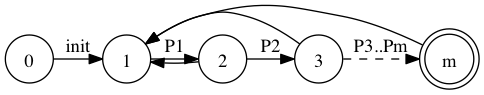
\includegraphics[width=.7\textwidth]{5.gv.png}
  \caption{Nonoverlappable patterns.}
\label{fig:5}
\end{figure}



\pagebreak

\end{document}